\documentclass[11pt]{article}
\usepackage[letterpaper, margin=1in, top=10mm]{geometry}
\usepackage{amsmath}
\usepackage{graphicx}
\usepackage{siunitx}
\usepackage{enumerate}
\usepackage{minted}
\usepackage{algpseudocode}
\usepackage[linesnumbered,vlined,ruled]{algorithm2e}
\usepackage[square,numbers]{natbib}
\usepackage{booktabs}
\usepackage{multirow}
\graphicspath{{./images}}
\begin{document}
    \title{PSRS Report}
    \author{Junwen Shen\\1770012\\junwen5@ualberta.ca}
    \date{\today}

    \maketitle

    \begin{abstract}
        Parallel sorting by regular sampling\cite{psrs:1993} is a parallel sorting design that uses regular sampling to balance the workload between threads.
        In this assignment, I implement the algorithm using \textit{C++} and \textit{pthread} and do a benchmark and analysis on the implementation.
    \end{abstract}


    \section{PSRS Implementations}
    \label{sec:section-1}
    Usually, engineers separate their \textit{C++} programs into header files and implementation files according to the design pattern of \textit{C++}.
    Thus, I also follow the same pattern to design the implementation of PSRS, where only public interfaces are exported in header files, and other functions are placed in \textit{.cpp} files, decorated by the static key word.
    The program contains two \textit{namespace}s (\textit{util} and \textit{psrs}) and the entry point \textit{main.cpp}, which is for test purposes only.
    In the following sub-section, I introduce each \textit{namespace} in details.

    \subsection{utils}
    \label{subsec:section-1-1}
    This \textit{namespace} is used for providing a utility class, \textit{Timer}\cite{timer:2012}, and two helper functions, namely, \textit{print\_vector}\cite{print_vector:2012} and \textit{format}\cite{string_format:2014}.
    The \textit{Timer} class is a template class that can let users measure duration by calling \textit{start} and \textit{stop} methods on its instance.
    Moreover, it is a \textit{std::chrono::steady\_clock} internally, which is most suitable for measuring intervals\cite{std_steady_clock:2022}. \textit{print\_vector} function is designed for debugging, it can print an input vector as a string series. \textit{format} function is a poly-fill for \textit{std::format}\cite{std_format:cpp20} as \textit{clang++14} marked this feature as incomplete\cite{std_format:2022} (\textit{clang++15} does not mention this feature, neither).

    \subsection{psrs}
    \label{subsec:section-1-2}
    This \textit{namespace} is used for exporting the public interface function, \textit{psrs}, which is exactly the implementation of the PSRS paper, and encapsulating other functions which are only used by \textit{psrs}.
    The function \textit{psrs} takes a reference of an integer vector, the number of threads, and a optional reference of an 64-bit integer vector to store runtime of each phase, and returns an sorted integer vector as the result, where the original vector remains unchanged.
    The following pseudo-code~\ref{alg:one} shows the workflow of \textit{psrs} function.
    The workflow of $parallel\_sort$ function in the \textit{psrs} function is described in the original paper, which contains four phases.
    Moreover, for measuring the total time in details, here I define two more phases, where Phase 0 is the initialization phase and Phase 5 is the collection and joining phase.
    The initialization phase generates payloads for each thread as well as some global variables stored in the \textit{Globals} class.
    The collection phase concatenates the array from each thread, and joins the threads.

    \begin{algorithm}
        \caption{PSRS Workflow}
        \label{alg:one}
        \SetKwFunction{Init}{initialize}
        \SetKwFunction{Create}{pthread\_create}
        \SetKwFunction{PSRS}{parallel\_sort}
        \SetKwFunction{Join}{pthread\_join}
        \SetKwInOut{Input}{input}\SetKwInOut{Output}{output}
        \Input{An unsorted array $V$ of size $s$; the number of threads $t$}
        \Output{A sorted array $V^{'}$}
        \BlankLine
        pthreads payloads $payloads \longleftarrow \phi$\\
        pthreads identifiers $pthreads \longleftarrow \phi$\\
        \For{$i\leftarrow 0$ \KwTo $t-1$}{
            \Init{$V$,\ $payloads[i]$}
        }
        \For{$i\leftarrow 1$ \KwTo $t-1$}{
            \Create{$pthreads[i]$,\ parallel\_sort, $payloads[i]$}
        }
        \PSRS{(void*)\&payloads[0]}\\
        result array $V^{'} \longleftarrow payloads[0].result$\\
        \For{$i\leftarrow 1$ \KwTo $t-1$}{
            $V^{'} = V^{'} \cup payloads[i].result$\\
            \Join{$pthreads[i]$}
        }
        \Return $V^{'}$
    \end{algorithm}


    \section{Experiments}
    \label{sec:section_2}
    In this section, I provide details of the setup of the experiments, which is used for evaluation the implementation of \textit{PSRS}.

    \subsection{Platform}
    \label{subsec:section_2_1}
    Here is the spec sheets of the platform for testing.
    \begin{itemize}
        \item CPU: Intel Core i7-12800H, 6 Performance Cores + 8 Efficiency Cores, 12 + 8 Threads (with Hyper-Threading enabled)
        \item OS: Windows 11 Enterprise 22H2 with WSL2 (Ubuntu 22.04, kernel: 5.15.57.1-microsoft-standard-WSL2)
        \item Compiler: Clang++15 with CXX standard of C++23
    \end{itemize}

    \subsection{Setup}
    \label{subsec:section-2-2}
    The sizes of arrays are 32M, 64M, 128M, 192M, 256M, 320M, where the contents are randomly generated by \textit{std::uniform\_int\_distribution} function ranging from \textit{INT32\_MIN} to \textit{INT32\_MAX} in uniform distribution.
    The numbers of threads are even numbers between 2 to 20.
    Each size runs 10 times and the result is the average of the last 5 runs.
    At the start of each run, the main function generates an vector of a certain size containing uniformly distributed random integers, and calls sequential sorting function on a copy of the vector, as the built-in sorting is in-place, then calls \textit{psrs} in a for-loop of different numbers of threads.
    Thus, In each run, the random generated data is the same for both sequential and parallel sorting functions.
    Because \textit{psrs} uses barrier synchronization, the elapsed time for each phase is the longest time among all threads, and the sum of the elapsed times of all phases is the total elapsed time of \textit{psrs}.
    Therefore, every thread records and reports its own elapsed time of every phase, and the main thread calculates the actual elapsed time of each phase.
    At last, the correctness can be validated by comparing the copy sorted by the built-in sequential function and the data returned by \textit{psrs}.


    \section{Results}
    \label{sec:section-3}

    \begin{figure}[htbp]
        \centering
        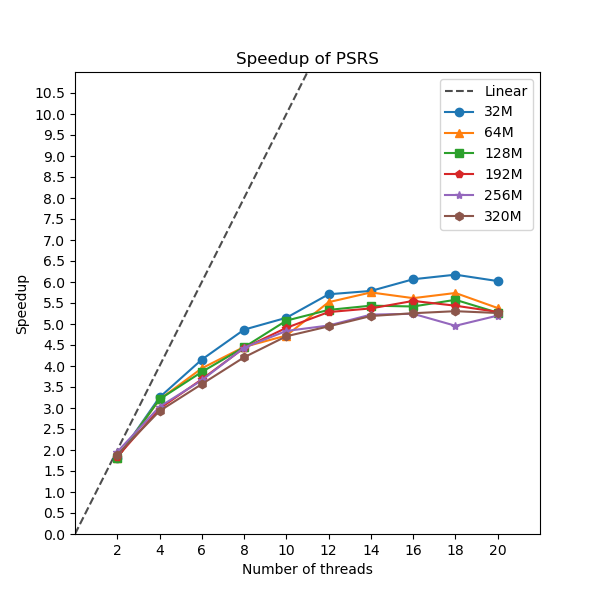
\includegraphics[width=0.5\textwidth]{speedup.png}
        \caption{Speedup of PSRS}
        \label{fig:speedup}
    \end{figure}

    \begin{table}[htbp]
        \centering
        \resizebox{\columnwidth}{!}{%
            \begin{tabular}{@{}|c|ccccccccccc|@{}}
                \toprule
                \multirow{3}{*}{sizes/threads} &
                \multicolumn{11}{c|}{\multirow{2}{*}{\begin{tabular}[c]{@{}c@{}}
                                                         Sorting Times\\ (in seconds)
                \end{tabular}}} \\
                &
                \multicolumn{11}{c|}{} \\ \cmidrule(l){2-12}
                &
                \multicolumn{1}{c|}{1} &
                \multicolumn{1}{c|}{2} &
                \multicolumn{1}{c|}{4} &
                \multicolumn{1}{c|}{6} &
                \multicolumn{1}{c|}{8} &
                \multicolumn{1}{c|}{10} &
                \multicolumn{1}{c|}{12} &
                \multicolumn{1}{c|}{14} &
                \multicolumn{1}{c|}{16} &
                \multicolumn{1}{c|}{18} &
                20 \\ \midrule
                32M &
                \multicolumn{1}{c|}{2.263} &
                \multicolumn{1}{c|}{1.252} &
                \multicolumn{1}{c|}{0.695} &
                \multicolumn{1}{c|}{0.545} &
                \multicolumn{1}{c|}{0.465} &
                \multicolumn{1}{c|}{0.440} &
                \multicolumn{1}{c|}{0.397} &
                \multicolumn{1}{c|}{0.391} &
                \multicolumn{1}{c|}{0.373} &
                \multicolumn{1}{c|}{0.367} &
                0.376 \\ \midrule
                64M &
                \multicolumn{1}{c|}{4.890} &
                \multicolumn{1}{c|}{2.697} &
                \multicolumn{1}{c|}{1.526} &
                \multicolumn{1}{c|}{1.239} &
                \multicolumn{1}{c|}{1.098} &
                \multicolumn{1}{c|}{1.035} &
                \multicolumn{1}{c|}{0.886} &
                \multicolumn{1}{c|}{0.85} &
                \multicolumn{1}{c|}{0.871} &
                \multicolumn{1}{c|}{0.852} &
                0.909 \\ \midrule
                128M &
                \multicolumn{1}{c|}{9.963} &
                \multicolumn{1}{c|}{5.508} &
                \multicolumn{1}{c|}{3.106} &
                \multicolumn{1}{c|}{2.582} &
                \multicolumn{1}{c|}{2.241} &
                \multicolumn{1}{c|}{1.961} &
                \multicolumn{1}{c|}{1.867} &
                \multicolumn{1}{c|}{1.833} &
                \multicolumn{1}{c|}{1.839} &
                \multicolumn{1}{c|}{1.787} &
                1.891 \\ \midrule
                192M &
                \multicolumn{1}{c|}{16.289} &
                \multicolumn{1}{c|}{8.867} &
                \multicolumn{1}{c|}{5.458} &
                \multicolumn{1}{c|}{4.422} &
                \multicolumn{1}{c|}{3.678} &
                \multicolumn{1}{c|}{3.318} &
                \multicolumn{1}{c|}{3.083} &
                \multicolumn{1}{c|}{3.033} &
                \multicolumn{1}{c|}{2.935} &
                \multicolumn{1}{c|}{2.997} &
                3.081 \\ \midrule
                256M &
                \multicolumn{1}{c|}{22.303} &
                \multicolumn{1}{c|}{11.405} &
                \multicolumn{1}{c|}{7.362} &
                \multicolumn{1}{c|}{6.093} &
                \multicolumn{1}{c|}{5.025} &
                \multicolumn{1}{c|}{4.614} &
                \multicolumn{1}{c|}{4.493} &
                \multicolumn{1}{c|}{4.27} &
                \multicolumn{1}{c|}{4.254} &
                \multicolumn{1}{c|}{4.499} &
                4.289 \\ \midrule
                320M &
                \multicolumn{1}{c|}{28.101} &
                \multicolumn{1}{c|}{14.894} &
                \multicolumn{1}{c|}{9.593} &
                \multicolumn{1}{c|}{7.873} &
                \multicolumn{1}{c|}{6.679} &
                \multicolumn{1}{c|}{5.969} &
                \multicolumn{1}{c|}{5.684} &
                \multicolumn{1}{c|}{5.415} &
                \multicolumn{1}{c|}{5.346} &
                \multicolumn{1}{c|}{5.297} &
                5.341 \\ \bottomrule
            \end{tabular}%
        }
        \caption{Sorting Times}
        \label{tab:sorting-times}
    \end{table}
    \begin{table}[htbp]
        \centering
        \resizebox{\columnwidth}{!}{%
            \begin{tabular}{|c|cccccccccc|}
                \hline
                \multirow{3}{*}{Phase/threads} &
                \multicolumn{10}{c|}{\multirow{2}{*}{\begin{tabular}[c]{@{}c@{}}
                                                         Sorting Times\\ (in microseconds)
                \end{tabular}}} \\
                &
                \multicolumn{10}{c|}{} \\ \cline{2-11}
                &
                \multicolumn{1}{c|}{2} &
                \multicolumn{1}{c|}{4} &
                \multicolumn{1}{c|}{6} &
                \multicolumn{1}{c|}{8} &
                \multicolumn{1}{c|}{10} &
                \multicolumn{1}{c|}{12} &
                \multicolumn{1}{c|}{14} &
                \multicolumn{1}{c|}{16} &
                \multicolumn{1}{c|}{18} &
                20 \\ \hline
                0 &
                \multicolumn{1}{c|}{290379} &
                \multicolumn{1}{c|}{195223} &
                \multicolumn{1}{c|}{211537} &
                \multicolumn{1}{c|}{213171} &
                \multicolumn{1}{c|}{219143} &
                \multicolumn{1}{c|}{216593} &
                \multicolumn{1}{c|}{215966} &
                \multicolumn{1}{c|}{218809} &
                \multicolumn{1}{c|}{216825} &
                226122 \\ \hline
                1 &
                \multicolumn{1}{c|}{13067073} &
                \multicolumn{1}{c|}{8102512} &
                \multicolumn{1}{c|}{6392375} &
                \multicolumn{1}{c|}{5142978} &
                \multicolumn{1}{c|}{4348529} &
                \multicolumn{1}{c|}{4008446} &
                \multicolumn{1}{c|}{3663934} &
                \multicolumn{1}{c|}{3516166} &
                \multicolumn{1}{c|}{3346533} &
                3336392 \\ \hline
                2 &
                \multicolumn{1}{c|}{1} &
                \multicolumn{1}{c|}{2} &
                \multicolumn{1}{c|}{2} &
                \multicolumn{1}{c|}{3} &
                \multicolumn{1}{c|}{4} &
                \multicolumn{1}{c|}{6} &
                \multicolumn{1}{c|}{8} &
                \multicolumn{1}{c|}{12} &
                \multicolumn{1}{c|}{15} &
                20 \\ \hline
                3 &
                \multicolumn{1}{c|}{183521} &
                \multicolumn{1}{c|}{136226} &
                \multicolumn{1}{c|}{130268} &
                \multicolumn{1}{c|}{138662} &
                \multicolumn{1}{c|}{142625} &
                \multicolumn{1}{c|}{148758} &
                \multicolumn{1}{c|}{153677} &
                \multicolumn{1}{c|}{143449} &
                \multicolumn{1}{c|}{143480} &
                139049 \\ \hline
                4 &
                \multicolumn{1}{c|}{1075799} &
                \multicolumn{1}{c|}{840668} &
                \multicolumn{1}{c|}{768302} &
                \multicolumn{1}{c|}{766295} &
                \multicolumn{1}{c|}{846212} &
                \multicolumn{1}{c|}{896549} &
                \multicolumn{1}{c|}{936764} &
                \multicolumn{1}{c|}{984962} &
                \multicolumn{1}{c|}{1061393} &
                1130113 \\ \hline
                5 &
                \multicolumn{1}{c|}{277203} &
                \multicolumn{1}{c|}{317938} &
                \multicolumn{1}{c|}{370255} &
                \multicolumn{1}{c|}{417930} &
                \multicolumn{1}{c|}{412609} &
                \multicolumn{1}{c|}{413803} &
                \multicolumn{1}{c|}{444231} &
                \multicolumn{1}{c|}{482446} &
                \multicolumn{1}{c|}{528577} &
                508934 \\ \hline
                Total &
                \multicolumn{1}{c|}{14893976} &
                \multicolumn{1}{c|}{9592569} &
                \multicolumn{1}{c|}{7872739} &
                \multicolumn{1}{c|}{6679039} &
                \multicolumn{1}{c|}{5969122} &
                \multicolumn{1}{c|}{5684155} &
                \multicolumn{1}{c|}{5414580} &
                \multicolumn{1}{c|}{5345844} &
                \multicolumn{1}{c|}{5296823} &
                5340630 \\ \hline
            \end{tabular}%
        }
        \caption{Sorting Times in Each phase (size = 320M)}
        \label{tab:sorting-times-in-phase}
    \end{table}

    Figure~\ref{fig:speedup} is the speedup graph and Table~\ref{tab:sorting-times} is the corresponding elapsed time of each size with certain number of threads.
    Moreover, Table~\ref{tab:sorting-times-in-phase} shows the distribution of elapsed time in each phase with different number of threads, where the size of the array to sort is 320M. It is obvious that the maximum speedup is 5.751 with 14 threads at 64M, and the implementation slows down for more than 16 threads.
    More importantly, the diminishing returns happen after more than 6 threads. \\
    From the breakdown of execution times according to phases, the elapsed time for Phase 1 decreased significantly from 2 threads till 6 threads, and for Phase 2 is barely noticeable.
    This is also the reason why I choose microsecond to be the unit for Table~\ref{tab:sorting-times-in-phase} instead of millisecond or seconds like in Table~\ref{tab:sorting-times}.
    However, it does increase as the number of threads increases as expected.
    Moreover, for other phases, the execution time increases as the number of threads increases.
    Although Phase 0 and 5 defined in Section~\ref{subsec:section-1-2} are shorter comparing to Phase 1 and 4, they both contribute a noteworthy amount of execution time.


    \section{Analysis}
    \label{sec:section-4}
    \begin{itemize}
        \item Phase 1 is where local data is sorted.
        Since the time complexity of comparison sorting is at least $\mathcal{O}(n\log n)$, the only way to reducing the run-time is reduce the amount of data for each threads, which is why increasing the number of threads leads to decrement of execution time as long as one physical core execute only one thread.
        Context switching creates a huge amount of overheads.
        Phase 4 is similar, the workload of merging is reduced by increasing the number of threads.
        \item Phase 2 is purely sequential and it will become to the bottleneck when the number of threads increases according to Amdahl's Law.
        However, in this experiment, the number of threads is too small to make it to be the bottleneck, and the increasing trend may also be affected by non-determinism.
        \item The main propose of Phase 3 is partitioning the local data and distributing the partitions, which mainly depends on the number of threads.
        Moreover, Phase 0 and Phase 5 also depends on the number of threads only.
        Therefore, the execution times of these phases have the same trend.
        They may be affected by non-determinism as well, due to the relatively short execution time.
    \end{itemize}


    \section{Limitations}
    \label{sec:section-5}
    \begin{itemize}
        \item \textit{pthread} vs \textit{std::thread} (proposed in \textit{C++11}) \\ The API and implementation of pthread (POSIX thread) are generally available on many UNIX/UNIX-like POSIX-conformant operating systems.
        However, it is not available on Windows directly\cite{pthread}.
        Windows has its own multi-threading API. \textit{C++} standard library introduced \textit{std::thread} since \textit{C++11}.
        It provides a higher abstraction of multi-threading APIs, which is cross-platform.
        The implementation of \textit{PSRS} in this report uses \textit{pthread} only.
        In order to compile and run tests on Windows, one option is rewriting it by using \textit{std::thread}.
        \item Heterogeneous CPU Topology \\ Heterogeneous CPU topology is a system design that all cores use the same instruction-set architectures, but the speed of cores vary\cite{heterogeneous}.
        Intel produced its 12th generation CPU in this design to provide better power efficiency.
        Although the main purpose of regular sampling in \textit{PSRS} is balancing the load between threads, scheduling the same amount of data between performance-cores and efficiency-cores is not actually balancing.
        Therefore, the results of the experiments may be affected by the different computation powers between different cores.
    \end{itemize}

    \bibliographystyle{abbrvnat}
    \bibliography{refs}

\end{document}
